% 2002 年上海理科第 15 题：函数图象选项示意
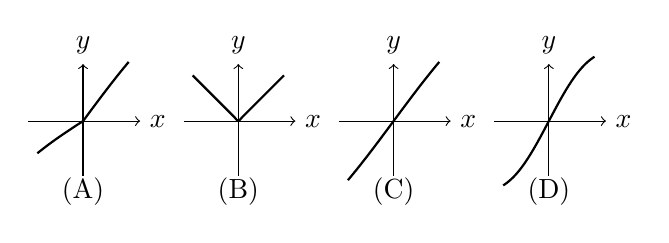
\begin{tikzpicture}[scale=0.58]
  \foreach \shift/\lab in {0/A,3.4/B,6.8/C,10.2/D} {
    \begin{scope}[xshift=\shift cm]
      \draw[->] (-1.2,0)--(1.25,0) node[right] {$x$};
      \draw[->] (0,-1.2)--(0,1.25) node[above] {$y$};
      \node at (0,-1.55) {(\lab)};
    \end{scope}
  }
  \draw[thick, domain=-1:1, smooth] plot ({\x},{\x+0.35*sin(deg(abs(\x)))});
  \draw[thick, domain=-1:1, smooth, xshift=3.4cm] plot ({\x},{abs(\x)});
  \draw[thick, domain=-1:1, smooth, xshift=6.8cm] plot ({\x},{\x+0.35*sin(deg(\x))});
  \draw[thick, domain=-1:1, smooth, xshift=10.2cm] plot ({\x},{\x+0.45*sin(deg(2*\x))});
\end{tikzpicture}
